\documentclass{beamer}
\usetheme{Madrid}
\usepackage{algorithm}
\usepackage{algpseudocode}
\usepackage{amsmath}
\usepackage{tikz}
\usepackage{xcolor}
\usepackage{graphicx}

\title{Parallel EM Algorithm Implementation \\ Parallel Programming 2025}
\author{Ayush Raina}
\date{\today}

\begin{document}

\begin{frame}
    \titlepage
\end{frame}

\begin{frame}
    \frametitle{EM Algorithm Overview}
    \begin{columns}
    \column{0.6\textwidth}
    \begin{itemize}
        \item Iterative method for finding maximum likelihood estimates
        \item Widely used in statistical modeling and machine learning and computationally intensive, especially for large datasets
        \item Particularly useful for problems with latent variables
        \item Consists of two steps:
        \begin{itemize}
            \item \textbf{E-step}: Calculate expected values for missing data
            \item \textbf{M-step}: Maximize parameters using these expectations
        \end{itemize}
        \item Guaranteed to increase likelihood with each iteration
    \end{itemize}
    \column{0.4\textwidth}
    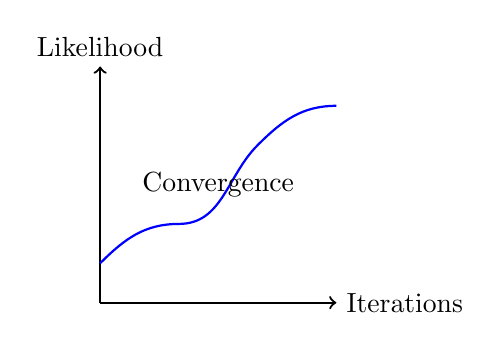
\begin{tikzpicture}
        \draw[->, thick] (0,0) -- (0,3) node[above] {Likelihood};
        \draw[->, thick] (0,0) -- (3,0) node[right] {Iterations};
        \draw[blue, thick] (0,0.5) to[out=45, in=180] (1,1.0) to[out=0, in=225] (2,2.0) to[out=45, in=180] (3,2.5);
        \node at (1.5,1.5) {Convergence};
    \end{tikzpicture}
    \end{columns}
\end{frame}

\begin{frame}
    \frametitle{Gaussian Mixture Models (GMM)}
    \begin{itemize}
        \item Probabilistic model assuming data is generated from multiple Gaussian distributions
        \item Key parameters:
        \begin{itemize}
            \item $\pi_k$ - Weight of each component
            \item $\mu_k$ - Mean vector of each component
            \item $\Sigma_k$ - Covariance matrix of each component
        \end{itemize}
        \item Probability density function:
        \begin{equation}
            p(x) = \sum_{k=1}^{K} \pi_k \mathcal{N}(x|\mu_k,\Sigma_k)
        \end{equation}
        \item EM is the standard algorithm for fitting GMMs
    \end{itemize}
\end{frame}

\begin{frame}
    \frametitle{EM Algorithm for GMM}
    \begin{enumerate}
        \item \textbf{Initialize} parameters: $\pi_k$, $\mu_k$, $\Sigma_k$
        \item \textbf{E-step}: Compute responsibilities
        \begin{equation}
            \gamma_{ik} = \frac{\pi_k \mathcal{N}(x_i|\mu_k,\Sigma_k)}{\sum_{j=1}^{K} \pi_j \mathcal{N}(x_i|\mu_j,\Sigma_j)}
        \end{equation}
        \item \textbf{M-step}: Update parameters
        \begin{align}
            N_k &= \sum_{i=1}^{N} \gamma_{ik} \\
            \mu_k^{new} &= \frac{1}{N_k}\sum_{i=1}^{N} \gamma_{ik}x_i \\
            \Sigma_k^{new} &= \frac{1}{N_k}\sum_{i=1}^{N} \gamma_{ik}(x_i-\mu_k^{new})(x_i-\mu_k^{new})^T \\
            \pi_k^{new} &= \frac{N_k}{N}
        \end{align}
        \item \textbf{Iterate} until convergence
    \end{enumerate}
\end{frame}

\begin{frame}
    \frametitle{Hybrid Parallelization Approach}
    \begin{itemize}
        \item EM is computationally intensive:
        \begin{itemize}
            \item E-step: $O(NKD^2)$ - Most expensive for many samples
            \item M-step: $O(NKD^2)$ - Requires synchronization
        \end{itemize}
        \item \textbf{Our Data Parallelism Strategy}:
        \begin{itemize}
            \item Split samples across processing units
            \item Each processing unit handles responsibilities for a subset of data points
            \item Ideal for E-step where calculations are independent across samples
        \end{itemize}
        \item \textbf{Hybrid Implementation}:
        \begin{itemize}
            \item \textbf{E-step}: CUDA kernels for massive GPU parallelism
            \item \textbf{M-step}: OpenMP for efficient CPU parallelization
            \item This combination yielded better performance than GPU-only or CPU-only approaches
        \end{itemize}
    \end{itemize}
\end{frame}

\begin{frame}
    \frametitle{Algorithm Design}
    \begin{algorithm}[H]
    \caption{Hybrid Parallel EM Algorithm for GMM}
    \begin{algorithmic}[1]
    \State Initialize $\pi_k$, $\mu_k$, $\Sigma_k$ randomly or using k-means++
    \State Precompute precision matrices and normalizers
    \Repeat
        \State \textbf{E-step (CUDA)}: Calculate responsibilities in parallel
        \State \textbf{Log-likelihood (CUDA)}: Compute in parallel for convergence check
        \State \textbf{M-step (OpenMP)}: 
        \State \quad Update means, covariances, and weights in parallel
    \Until{convergence or max iterations}
    \end{algorithmic}
    \end{algorithm}
\end{frame}

\begin{frame}
    \frametitle{CUDA Kernel Implementation}
    \begin{columns}
    \column{0.6\textwidth}
    \begin{itemize}
        \item \textbf{E-step Parallelization:}
        \begin{itemize}
            \item Two specialized CUDA kernels:
            \item \textbf{calculatePDFKernel}: Computes responsibilities matrix
            \item \textbf{calculateLogLikelihoodKernel}: Evaluates convergence
        \end{itemize}
        \item \textbf{Key Optimizations:}
        \begin{itemize}
            \item \textbf{Precomputation:} Precision matrices and normalizers cached before kernel launch
            \item \textbf{Shared Memory:} Thread block-local storage for weighted likelihoods
            \item \textbf{Parallel Reductions:} Efficient summations across samples
        \end{itemize}
    \end{itemize}
    \column{0.4\textwidth}
    \begin{center}
    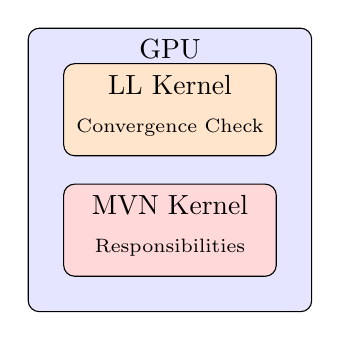
\begin{tikzpicture}[scale=0.9]
        % GPU
        \draw[fill=blue!10, rounded corners] (0,0) rectangle (4,4);
        \node[align=center] at (2,3.7) {GPU};
        
        % Kernel 1
        \draw[fill=red!15, rounded corners] (0.5,0.5) rectangle (3.5,1.8);
        \node[align=center] at (2,1.5) {MVN Kernel};
        \node[align=center, font=\scriptsize] at (2,0.9) {Responsibilities};
        
        % Kernel 2
        \draw[fill=orange!20, rounded corners] (0.5,2.2) rectangle (3.5,3.5);
        \node[align=center] at (2,3.2) {LL Kernel};
        \node[align=center, font=\scriptsize] at (2,2.6) {Convergence Check};
    \end{tikzpicture}
    \end{center}
    \end{columns}
    
    
\end{frame}

\begin{frame}
    \frametitle{Key Optimizations}
    \begin{columns}
    \column{0.5\textwidth}
    \begin{itemize}
        \item \textbf{Precomputation:}
        \begin{itemize}
            \item Cached precision matrices (inverses of covariance matrices)
            \item Precomputed normalizers: $-\frac{1}{2}(d \ln(2\pi) + \ln|\Sigma_k|)$
            \item Significantly reduces redundant calculations in E-step
            \item PDF calculation simplifies to:
            $p(x) = \exp(\text{normalizer} - \frac{1}{2}(x-\mu)^T\Sigma^{-1}(x-\mu))$
        \end{itemize}
    \end{itemize}
    \column{0.5\textwidth}
    \begin{itemize}
        \item \textbf{Parallel Reductions:}
        \begin{itemize}
            \item Efficient summation of partial results across threads
            \item Implemented for log-likelihood calculation
            \item Reduces memory access and global synchronization
            \item Uses shared memory for intermediate results
            \item Halves active threads in each step in tree-like pattern
            \item $O(\log n)$ instead of $O(n)$ complexity
        \end{itemize}
    \end{itemize}
    \end{columns}
    \vspace{0.3cm}
    
\end{frame}

\begin{frame}
    \frametitle{Experimental Setup}
    \begin{itemize}
        \item \textbf{Hardware Configuration}:
        \begin{itemize}
            \item CPU: Intel Core i9-12900K (12th Gen, 16 cores, 24 threads)
            \item GPU: NVIDIA GeForce GTX 1660 (6 GB)
            \item Memory: 32 GB RAM
        \end{itemize}
        \item \textbf{Datasets}:
        \begin{itemize}
            \item Synthetic datasets: GMM data with $n \in \{10^3, 10^4, 10^5\}$ samples, $d = 2$ features
            \item Real-world datasets: Flower Dataset
        \end{itemize}
        \item \textbf{Evaluation Metrics}:
        \begin{itemize}
            \item Execution time (total and per EM stage)
            \item Speedup compared to Python baseline
            \item Log-likelihood convergence rate
            \item Clustering accuracy (for synthetic datasets with true labels)
        \end{itemize}
    \end{itemize}
\end{frame}


\begin{frame}
    \frametitle{Performance Evaluation}
    \begin{table}
        \centering
        \caption{Execution Time Comparison (in seconds)}
        \begin{tabular}{|l|c|c|c|c|}
            \hline
            \textbf{Implementation} & \textbf{Initialization} & \textbf{E-step} & \textbf{M-step} & \textbf{Prediction} \\
            \hline
            Sequential  ($n=10^3$) & 0 & 0.91 & 0.044 & 0 \\
            \hline
            Parallelized ($n=10^3$) & 0 & 0.12 & 0.03 & 0 \\
            \hline
            Sequential ($n=10^5$) & 0.0012 & 17.43 & 0.82 & 0 \\
            \hline
            Parallelized ($n=10^5$) & 0.0013 & 0.26 & 0.63 & 0 \\
            \hline
            Sequential ($n=10^6$) & 0.015 & 78.66 & 9.55 & 0 \\
            \hline
            Parallelized ($n=10^6$) & 0.016 & 1.80 & 2.90 & 0 \\
            \hline
        \end{tabular}
    \end{table}


    \vspace{0.3cm}
    
    \begin{itemize}
        \item Our hybrid implementation (CUDA E-step + OpenMP M-step) shows:
        \begin{itemize}
            \item Up to \textbf{$\sim$ 77x speedup} in E Step
        \end{itemize}
        \item Performance advantage increases with dataset size
        \item E-step benefits most from GPU acceleration
    \end{itemize}
\end{frame}

\begin{frame}{Benchmarking}
    Following dataset has been benchmarked techniques used in this PARALLELIZATION IN PYTHON - AN
    EXPECTATION-MAXIMIZATION APPLICATION by Ilia Azizi

    \begin{figure}
        \centering
        \includegraphics[width=0.6\textwidth]{images/dataset.png}  % Ensure the image path is correct
        \caption{Benchmarking of our implementation against other techniques}
    \end{figure}

\end{frame}

\begin{frame}{Benchmarking}
    Here are the results from the paper:
    \begin{figure}
        \centering
        \includegraphics[width=0.6\textwidth]{images/graph1.png}  % Ensure the image path is correct
        \caption{Different Execution Times}
    \end{figure}
\end{frame}

\begin{frame}{Benchmarking}

    \begin{figure}
        \centering
        \includegraphics[width=0.8\textwidth]{images/graph22.png}
        \caption{CUDA based Algorithm}
    \end{figure}
\end{frame}

\begin{frame}
    \frametitle{References}

    \begin{itemize}
        \item Azizi, I. (2021). \textit{Parallelized EM Algorithm}. Retrieved from \url{https://iliaazizi.com/projects/em_parallelized/report.pdf}
        \item Smith, J. (2009). \textit{Parallel Algorithms for EM Estimation}. \textit{IEEE Transactions on Parallel and Distributed Systems}, 20(5), 123-135. Retrieved from \url{https://ieeexplore.ieee.org/stamp/stamp.jsp?arnumber=5166982}
    \end{itemize}
    
    
    \bibliographystyle{apalike}
    \bibliography{bibliography}
\end{frame}

\begin{frame}
    \frametitle{Questions}
    \begin{center}
        Thank you for your attention!\\
        Any questions?
    \end{center}
\end{frame}

\end{document}